\documentclass[aspectratio=169]{beamer}
\usetheme[faculty=phil]{fibeamer}
\usepackage{polyglossia}
\setmainlanguage{english} %% main locale instead of `english`, you
%% can typeset the presentation in either Czech or Slovak,
%% respectively.
\setotherlanguages{russian} %% The additional keys allow
%%
%%   \begin{otherlanguage}{czech}   ... \end{otherlanguage}
%%   \begin{otherlanguage}{slovak}  ... \end{otherlanguage}
%%
%% These macros specify information about the presentation
\title[AGLA2]{Analytical Geometry and Linear Algebra II, Lab 3} %% that will be typeset on the
\subtitle{Quiz \\ Four Fundametal Subspaces \\ \ 
         } %% title page.
\author{Oleg Bulichev}
%% These additional packages are used within the document:
\usepackage{ragged2e}  % `\justifying` text
\usepackage{booktabs}  % Tables
\usepackage{tabularx}
\usepackage{tikz}      % Diagrams
\usetikzlibrary{calc, shapes, backgrounds}
\usepackage{amsmath, amssymb}
\usepackage{url}       % `\url`s
\usepackage{listings}  % Code listings
% \usepackage{subfigure}
\usepackage{floatrow}
\usepackage{subcaption}
\usepackage{mathtools}
\usepackage{todonotes}
\usepackage{fontspec}
\usepackage{multicol}
\graphicspath{{resources/}}
\frenchspacing

\setbeamertemplate{caption}[numbered]
\usetikzlibrary{graphs}

% \usepackage[backend=biber,style=ieee,autocite=footnote]{biblatex}
% \addbibresource{biblio.bib}
% \DefineBibliographyStrings{english}{%
%   bibliography = {References},}

\newcommand{\oleg}[2][] {\todo[color=red, #1] {OLEG:\\ #2}}
\newcommand{\fbckg}[1]{\usebackgroundtemplate{\includegraphics[width=\paperwidth]{#1}}}%frame background

\usepackage[framemethod=TikZ]{mdframed}
\newcommand{\dbox}[1]{
\begin{mdframed}[roundcorner=3pt, backgroundcolor=yellow, linewidth=0]
\vspace{1mm}
{#1}
\vspace{1mm}
\end{mdframed}
}

\begin{document}
\fbckg{fibeamer/figs/title_page.png}
\frame[c]{\setcounter{framenumber}{0}
    \usebeamerfont{title}%
    \usebeamercolor[fg]{title}%
    \begin{minipage}[b][6.5\baselineskip][b]{\textwidth}%
        \textcolor{black}{\raggedright\inserttitle}
    \end{minipage}
    % \vskip-1.5\baselineskip

    \usebeamerfont{subtitle}%
    \usebeamercolor[fg]{framesubtitle}%
    \begin{minipage}[b][3\baselineskip][b]{\textwidth}
        \raggedright%
        \insertsubtitle%
    \end{minipage}
    \vskip.25\baselineskip
}
%   \frame[c]{\maketitle}

\fbckg{fibeamer/figs/common.png}

\begin{frame}[t]{Quiz}
    \framesubtitle{}
    \vspace{-0.3cm}
    1) Obtain $P$, $L$, $U$ matrices from $A$, using $PA=LU$ factorization.
    \begin{columns}[T,onlytextwidth]
        \begin{column}{0.49\textwidth}
            \begin{equation}
                A = \begin{bmatrix}
                    1 & 2  & 3  & 4  \\
                    5 & 6  & 7  & 8  \\
                    9 & 10 & 11 & 12
                \end{bmatrix}
            \end{equation}
        \end{column}
        \begin{column}{0.49\textwidth}
            \begin{equation}
                A = \begin{bmatrix}
                    1 & 4  & 0 & 0 \\
                    3 & 12 & 1 & 5 \\
                    2 & 8  & 1 & 5 \\
                    0 & 2  & 2 & 3
                \end{bmatrix}
            \end{equation}
        \end{column}
    \end{columns}
    \vspace{0.1cm}
\begin{columns}[T,onlytextwidth]
    \begin{column}{0.3\textwidth}
        2) For $\begin{bmatrix}
            1 & 2 & 3 & 5  \\
            2 & 4 & 8 & 12 \\
            3 & 6 & 7 & 13
        \end{bmatrix} x = \begin{bmatrix}b_1\\b_2\\b_3\end{bmatrix}$ \\
        for 5th point $Ax=[0,\ 6,\ -6]$
    \end{column}
    \begin{column}{0.7\textwidth}
        \begin{enumerate}
            \item Reduce $[A\ b]$ to $[U\ c]$, to reach a triangular system.
            \item Find the condition on $b_1$, $b_2$, $b_3$ to have a soultion.
            \item Describe the column space of $A$. Find the basis of the column space.
            \item Describe the nullspace of $A$. Declare free variables.
            \item Find a particular solution and the complete solution $x_p + x_n$
        \end{enumerate}
    \end{column}
\end{columns}
\end{frame}

% \section{Introduction}
% \begin{frame}[t]{\insertsectionhead}



\begin{frame}[t]{Task 1}
    \framesubtitle{}
    \begin{figure}[H]
        \centering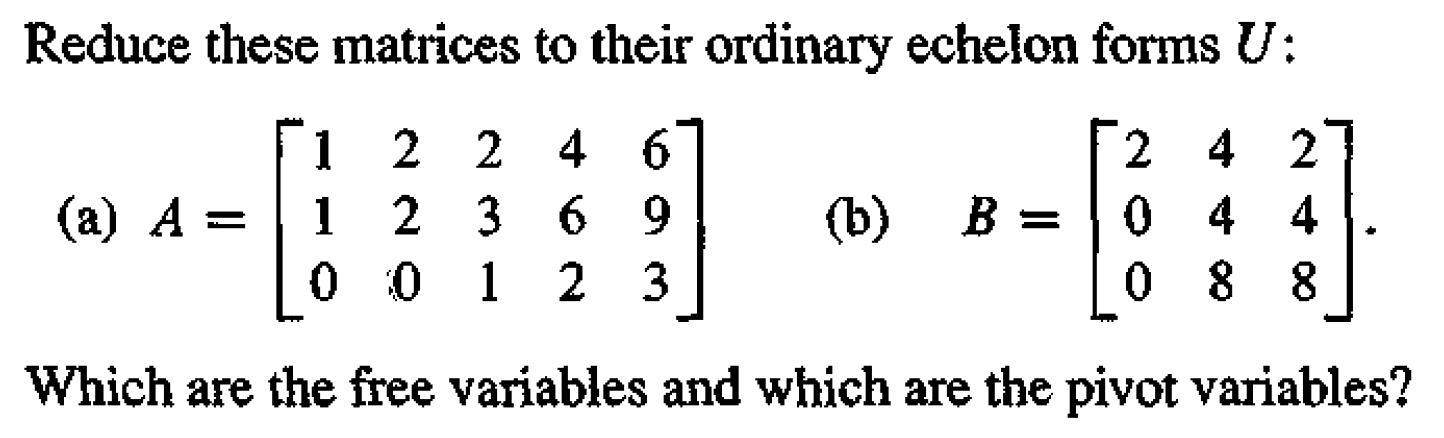
\includegraphics[height=3cm,width=1\textwidth,keepaspectratio]{1.png}
        % \caption{caption_name}
        \label{fig:1.png}
    \end{figure}
    \uncover<2->{
        \alert{\Large Answer}
        \begin{figure}[H]
            \centering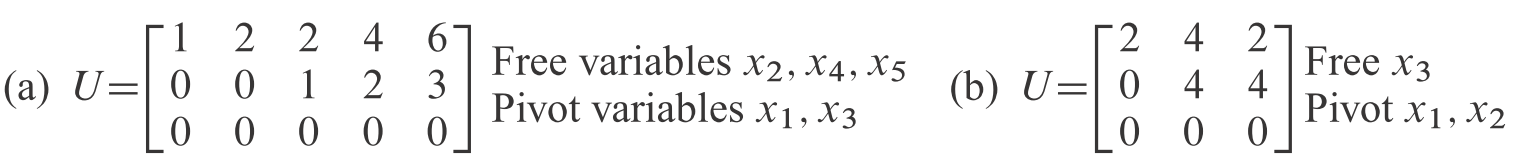
\includegraphics[height=3cm,width=1\textwidth,keepaspectratio]{1ans.png}
            % \caption{caption_name}
            \label{fig:1ans.png}
        \end{figure}
    }
\end{frame}

\begin{frame}[t]{Task 2}
    \framesubtitle{}
    \begin{figure}[H]
        \centering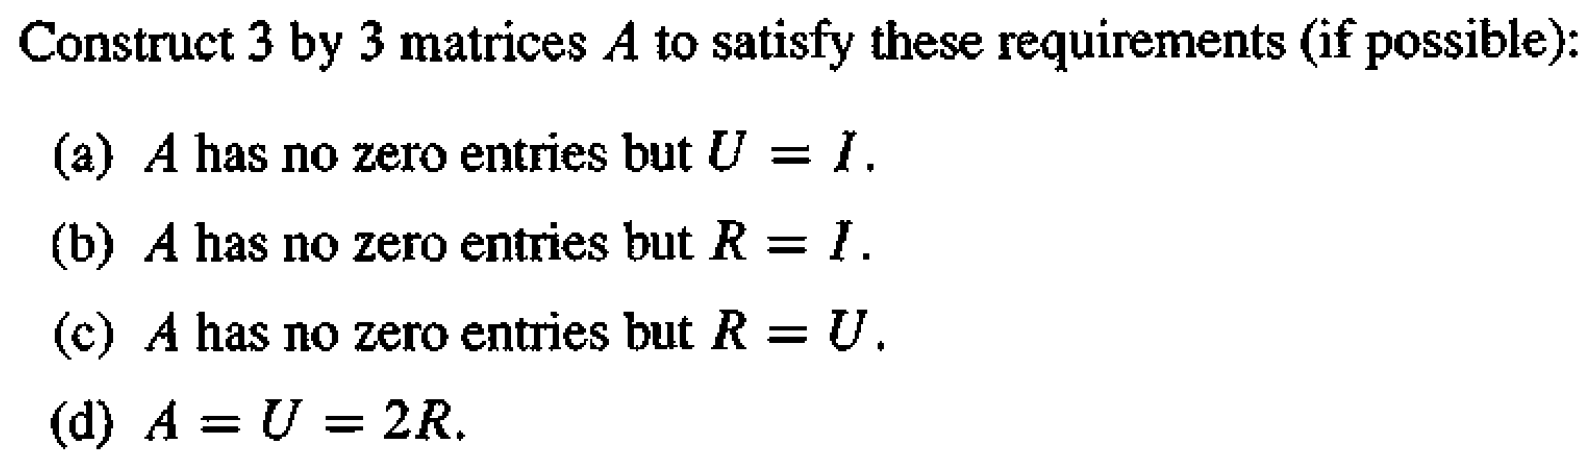
\includegraphics[height=3cm,width=1\textwidth,keepaspectratio]{2.png}
        % \caption{caption_name}
        \label{fig:2.png}
    \end{figure}
    \uncover<2->{
        \alert{\Large Answer}
        \begin{figure}[H]
            \centering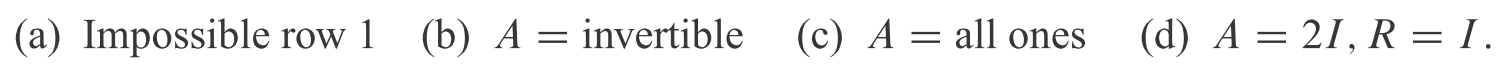
\includegraphics[height=3cm,width=1\textwidth,keepaspectratio]{2ans.png}
            % \caption{caption_name}
            \label{fig:2ans.png}
        \end{figure}
    }
\end{frame}

\begin{frame}[t]{Task 3}
    \framesubtitle{}
    \begin{figure}[H]
        \centering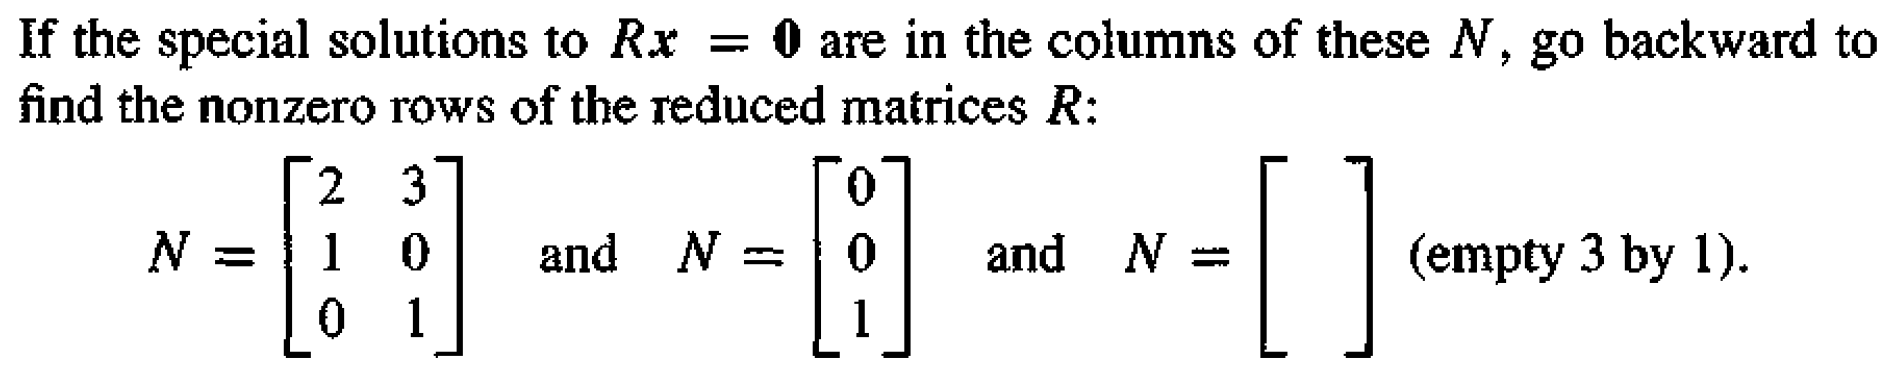
\includegraphics[height=3cm,width=1\textwidth,keepaspectratio]{3.png}
        % \caption{caption_name}
        \label{fig:3.png}
    \end{figure}
    \uncover<2->{
        \alert{\Large Answer}
        \begin{figure}[H]
            \centering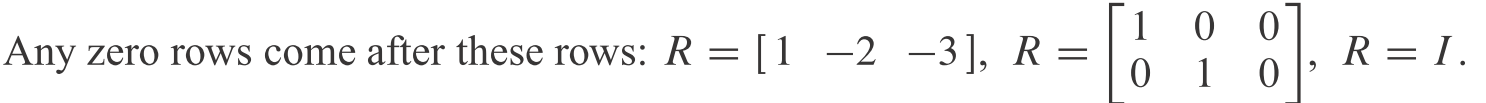
\includegraphics[height=3cm,width=1\textwidth,keepaspectratio]{3ans.png}
            % \caption{caption_name}
            \label{fig:3ans.png}
        \end{figure}
    }
\end{frame}

\begin{frame}[t]{Reference material}
    \framesubtitle{}
    \Large
    \begin{itemize}
        \item \href{https://www.youtube.com/watch?v=yjBerM5jWsc&list=PL49CF3715CB9EF31D&index=9}{Lecture 9 and 10}
        \item \textit{"Linear Algebra and Applications", pdf pages 139--149 }\\ The application of four fundamental subspaces in CS
        \item \href{https://youtu.be/yfj8uMwAgrI}{Matrix Transpose and the Four Fundamental Subspaces}\\ Video is about how $A$ transpose appeared
        \item \href{https://matworld.ru/calculator/matrix-calculator-1.php}{Matrix online calculator in russian}
    \end{itemize}
\end{frame}

\fbckg{fibeamer/figs/last_page.png}
\frame[plain]{}

\end{document}